\section{The Superstition of Reason}

\begin{wrapfigure}{rt}{.3\textwidth}
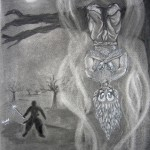
\includegraphics[width=.3\textwidth]{Vetal-150x150.jpg}
\end{wrapfigure}


To paraphrase a Scottish poet, perhaps no other word, other than those of \emph{Liberty} or \emph{Christ}, have been subject to as much abuse as the word ``\emph{Reason}``. These days the word \emph{Reason} has been defined to objectively exclude the very possibility of higher Intelligence, or higher Logos. At best, dialectical Reason (of the kind that American liberals imagined Socrates to be engaged in, illustrated by the career of Scott Buchanan\footnote{\url{http://en.wikipedia.org/wiki/Scott_Buchanan}}) is allowed to achieve the suspension of \emph{Aporia}. John Rawls\footnote{\url{http://en.wikipedia.org/wiki/John_Rawls}} embodied or re-embodied a lot of the vigor left in classical modern liberalism by restating Hobbes and Locke's contractual theory in a way that Buchanan might have found congenial, given as he was to attempts to re-invigorate the social ``federalism'' of the early American republic. This is the area which the great critic Richard Weaver termed ``the excluded middle'', and he argued that much of liberalism ``dances about in it''. At the other end is the view that ``reason is what the mind uses, and the mind is what the brain does'': this view is increasingly popular in a ``rational'' era. The term ``reason'' in either case (though far more malignantly in the latter) substitutes in such a way as to obliterate (like a lunar eclipse) the obviously solar presence of higher Reason. On the contrary, anyone who experiences an illumination (greater or lesser) finds that the experience is finding one's self, and simultaneously experiences finding something that is already thought (utterly rational) and yet utterly free (alive and imparting life and therefore freedom). So the sum of the experience is supra-rational. This would not seem to be such a controversial point, as it is well within the intellectual capacity of a hard-working twelve year old, but in the modern West, it appears to be so. It also happens to be the united and universal testimony of the best human beings of all higher cultures, and even of many of those which are not ``higher'', which explains why the burned out dregs of liberalism often turn to the lowest common denominator they can find among the outskirts of Tradition, in the form of the New Age or noble savagery.

In the tale of \textit{Vikrama and Vitala}\footnote{\url{http://en.wikipedia.org/wiki/Baital_Pachisi}}, the king captures a vampire at the behest of a treasonous tantric sorcerer, who intends to use both of them to overthrow legitimate authority. The tale is instructive, as it points out that illegitimacy lurks not in the most obvious evil, but rather in the moralistic facade of the cunning and clever, who see an opportunity for advancement at the expense of those who do not ``know''. The king is saved by listening to the captive vampire, who reveals the plan of the sorcerer and suggests a manner to overcome him. In this fable, it is seen how superstitious ``Reason'' has actually become, because it denies both the authority of the Emperor and attempts to master the black arts in Saruman-like fashion in order to augment personal power. Is it not superstitious to deny the fullness of God's Creation, and to make taboo and totem out of whatever is accidentally congenial to one's bent? The natural authority of the secular ruler and realm of the supernatural are both to be subjugated to the desires of the sorcerer-state, a theory of politics which one actually finds expounded in the works of Culianu\footnote{\url{http://thearchdruidreport.blogspot.com/2011/10/plutos-republic.html}}. We can see how ``Reason'' in the modern world, both as the prostitute and the ostensible mistress of Science and Justice, is similar to the thaumaturgic tantric-sorcerer of the Legend.

As great a poet, humanist, and thinker as Voltaire was seduced by the charms of secular thaumaturgy. It is a well known fact that the sublimated erotic rivalries of great thinkers and rulers who are legitimate often become mimicked in miniscule through their disciples, who are unable to appreciate the full scope of their work, but certainly key in on the tensions of their desires within the rivalries. Phillip Rieff drew attention to this in his work on \emph{Second Death}\footnote{\url{http://www.amazon.com/Fellow-Teachers-Culture-Second-Death/dp/0226716449}}. Thus, \emph{Voltaire's Bastards}\footnote{\url{http://www.amazon.com/Voltaires-Bastards-Dictatorship-Reason-West/dp/1476718962/ref=sr_1_1?s=books\&ie=UTF8\&qid=1423888644&sr=1-1&keywords=voltaires+bastards}} come to dominate the mental landscape of the West. Poor Voltaire wrote entertaining fiction like Candide, but never really (and self-confessed this) came to resolve the problem of Evil, and had to be content with living like a parasite off the ruins of an Age he helped to destroy. Don't end up like him.

The only way out this impasse is not to partake of the fighting in the rubble and ruin of the Western mental landscape, which is at this point dominated by the bastards of Reason in various titanic forms: there are the scientific crowds who can't accept something unless it can be explained in its most reductive terms, there are the masses of political factions who believe that the one burning question right now is to catalyze some form of resistance to the spread of whatever alien idea they define themselves in opposition to, there are the groups of people who endeavor to ``dance about in the excluded middle'' and prop things up by appealing to something along the lines of
\emph{Religion Within the Limits of Reason Alone}\footnote{\url{https://en.wikipedia.org/wiki/John_Toland}}, etc., etc.

No wonder Gornahoor lays so much emphasis on avoiding dialectical quarrels with those who don't share aims and principles, getting things right at the foundation, and putting practice into theory (and vice versa) from the beginning, so that one is most assuredly not at the behest or beholding of a salary, an occupation, or a career of some sorts. These webs of A influences (legitimate in their own way, but self-canceling in the sense that they operate mechanically through humans under their sway) will eventually reduce what they master to rubble, much like the current landscape seems to be vividly illustrating.

Those who want to find something that Russell Kirk called \emph{The Permanent Things} would do well to model their lives more on the life of a king Vikrama, who was brave enough to face vampires, and wise enough to listen to what he learned and avoid the trap that had been set for him. A young man could do much worse than aspire to the heroic and respect the supernatural -- or, as Jesus put it, to be wise as a serpent, but innocent as a dove. The alternatives seem to be being part of the Sheeple, or aspiring to rule over them as a sorcerer.


\flrightit{Posted on 2015-02-13 by Logres}

